% !TeX spellcheck = en_GB
% !TeX encoding = UTF-8
\documentclass[oneside,a4paper]{article}
\usepackage{makeidx}
\usepackage{float}
\usepackage{graphicx}
\usepackage{smartref}
\usepackage[hidelinks]{hyperref}
\usepackage{xcolor}
\usepackage{xspace}
\hypersetup{
	colorlinks,
	linkcolor={red!50!black},
	citecolor={blue!50!black},
	urlcolor={blue!80!black}
}
\graphicspath{ {images/} }

\newcommand{\wlversion}{0.16.2}
\newcommand{\guidefor}{For Eve Incursion Waitlist: \wlversion\xspace}

\newcommand{\piccross}{
\includegraphics{cross.png}\xspace}
\newcommand{\picbell}{
\includegraphics{bell.png}\xspace}
\newcommand{\picfits}{
\includegraphics{fits.png}\xspace}
\newcommand{\picconvo}{
\includegraphics{convo.png}\xspace}
\newcommand{\picinvite}{
\includegraphics{invite.png}\xspace}
\newcommand{\picfleetsetting}{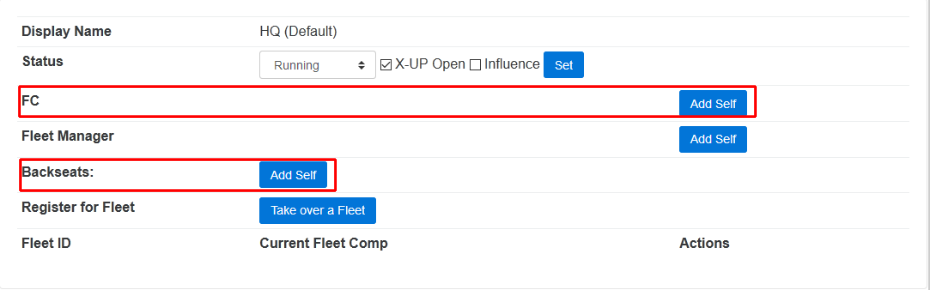
\includegraphics[width=\textwidth]{takeover-fc.png}\xspace}
\newcommand{\picset}{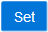
\includegraphics{set.png}\xspace}
\newcommand{\picremove}{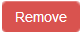
\includegraphics[scale=0.5]{remove.png}\xspace}
\newcommand{\picassignedfleet}{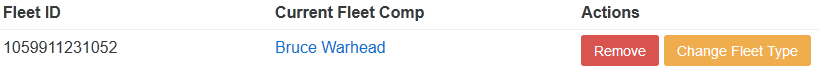
\includegraphics[width=\textwidth]{assigned-fleet.png}}
\newcommand{\picchangetype}{
\includegraphics[scale=0.5]{change-type.png}}
\newcommand{\picsettype}{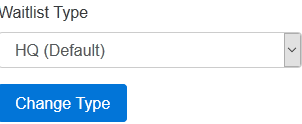
\includegraphics[scale=0.5]{set-type.png}}
\newcommand{\picteamspeaksettings}{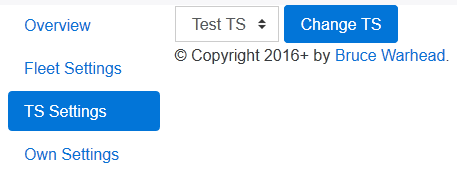
\includegraphics{teamspeak-settings.png}}
\newcommand{\picchangets}{
\includegraphics[scale=0.5]{change-ts.png}}
\newcommand{\picownsettings}{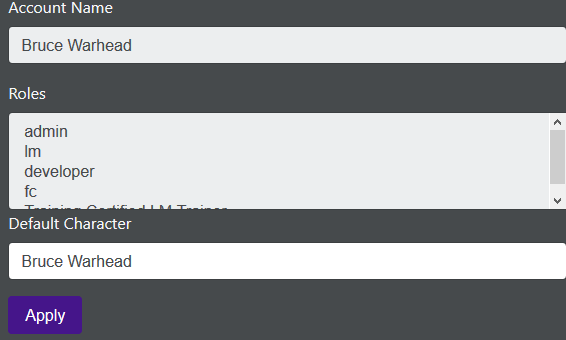
\includegraphics[width=\textwidth]{own-settings.png}}
\newcommand{\picapply}{
\includegraphics[scale=0.5]{apply.png}}

\title{Eve Incursion Waitlist Manual}
\author{Bruce Warhead and Beryl Slanjava}



\makeindex 

\setcounter{tocdepth}{3}

\begin{document}

\maketitle
\begin{center}
\guidefor
\end{center}


\tableofcontents

\newpage


%%%%%%%%%%%%%%%%%%%%%%%%%%%%%%%%%%%%%%%%%%%%%%%%%%%%%%%%%%%%%%%%%%%%
\section{FC-/Backseat-Guide}
\subsection{Starting or Takingover Fleet}
\subsubsection{As Fleetmanager}
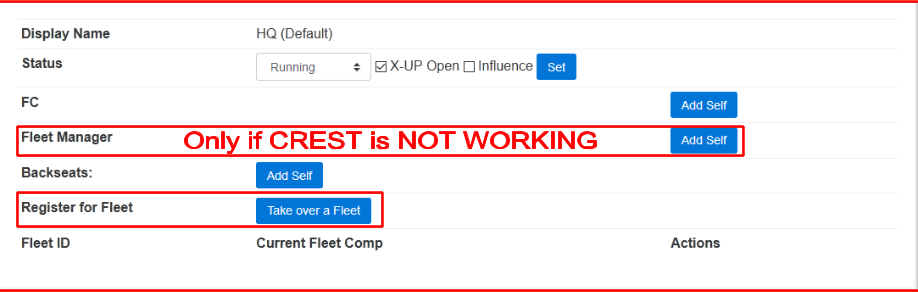
\includegraphics[width=\textwidth]{takeover-fleetmanager.png}
\begin{enumerate}
	\item If the eve api is not working, set yourself manually as fleet manager via 
\includegraphics[scale=0.5]{add-self.png}
	\item Start fleet and copy your external fleet link into the Waitlist when requested after pressing 
\includegraphics[scale=0.5]{take-over-fleet.png}
	\item  You will be taken to CCP's SSO-Login page to confirm who you are and to allow the Waitlist to interact with your fleet.
\end{enumerate}
If you are taking over an existing fleet, it will set you as the new fleet manager and you are done.
If you are starting a new Fleet, the following additional steps are needed
\begin{enumerate}
	\item After granting the Waitlist access we will request the external fleet link again and confirm what fleet you are in HQ/AS or VG’s. Depending on this the Auto-Fleet-Setup builds your squads and sets the MOTD.	
	\item Afterwards match your In-Game Squads to the Waitlist-Group lists. Ie. Logi-list to Logi-Squad, DPS-list to DPS-Squad
\end{enumerate}
\subsubsection{As FC or Backseat}
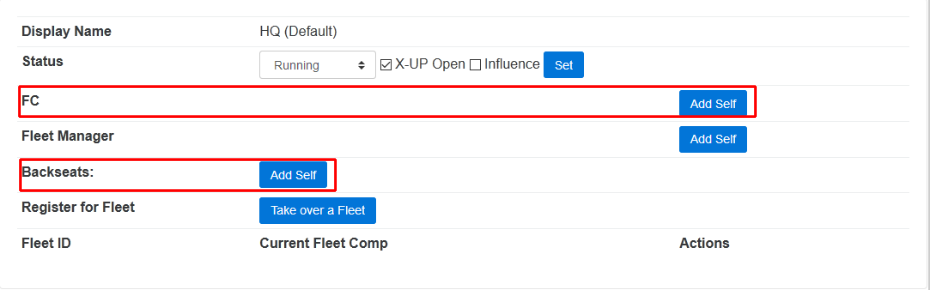
\includegraphics[width=\textwidth]{takeover-fc.png}
\begin{enumerate}
	\item If you are FC add your self in the FC-Row by pressing 
\includegraphics[scale=0.5]{add-self.png}
	\item If you are Backseat to a T-Badge add your self in the Backseats-Row by pressing 
\includegraphics[scale=0.5]{add-self.png} there
	\item If characters are still listed that are not Backseating/Fleetcommanding any more please use the \piccross to the right of their name to remove them (They should have done that when leaving through)
\end{enumerate}

\subsection{Leaving Fleet}
\subsubsection{As Fleetmanager}
If the eveapi is working and used you need to do Nothing, when the other Person takes the fleet, it will automatically replace you as Fleetmanager.
If the eveapi was not working, and the manual way of setting a Fleetmanager was used, you need to remove yourself from it by pressing the \piccross to the right of your name.

\subsubsection{As FC or Backseat}
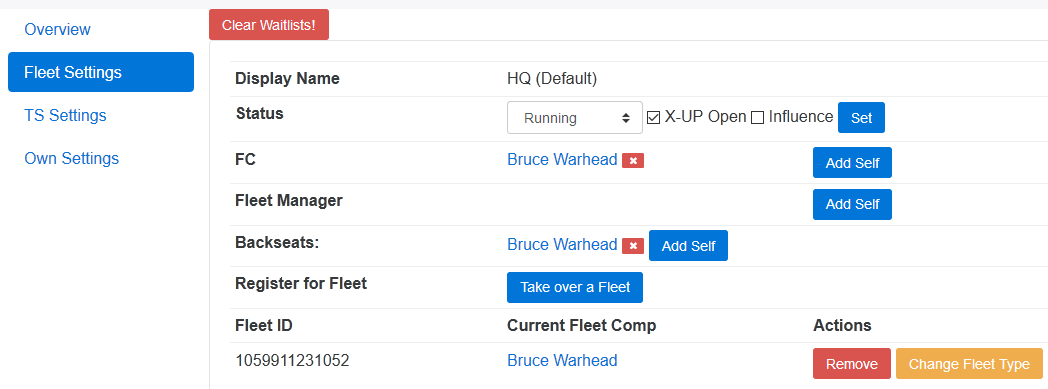
\includegraphics[width=\textwidth]{leaving-backseat.png}
When you are leaving fleet and you where the Fleetcommander or Backseat remove yourself from the FC- or Backseats-Row using the \piccross to the right of your name.


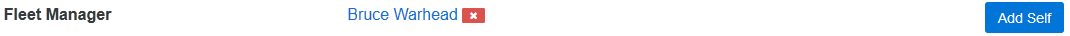
\includegraphics[width=\textwidth]{manual-fleet-manager.png}

\subsection{Checking Fits on X-UP}
\begin{figure}[H]
	\centering
	\caption{Entry on the X-UP list}
	\label{pic:xup-entry}
	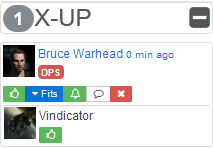
\includegraphics[]{xup-list.png}
\end{figure}

\begin{itemize}
	\item 
\includegraphics{fits.png} Shows/Hides the fittings
	\item 
\includegraphics{thumbup.png} below the portrait accepts all fits from this character
	\item 
\includegraphics{bell.png} Sends a Notification (make the gong go off) and poke (with the message that the FC wants something from them) on TeamSpeak if they are on there and their Charactername matches exactly (case sensitive and no additions)
	\item \piccross Remove a entry from X-UP, this does not affect that characters entries in the Waitlists!
	\item 
\includegraphics{thumbup.png} NEXT to a FIT, allows to approve this single fit, without approving an of the other fits. To deny specific fits, you accept all fits that you want to accept using 
\includegraphics{thumbup.png} next to the fit and then use 
	\piccross to remove the X-UP Entry.
	\item Click anywhere on a fit except the 
\includegraphics{thumbup.png} to open a Fittingwindow (Figure \ref{pic:fittingwindow}).
\end{itemize}
\begin{figure}
	\centering
	\caption{Fittingwindow}
	\label{pic:fittingwindow}
	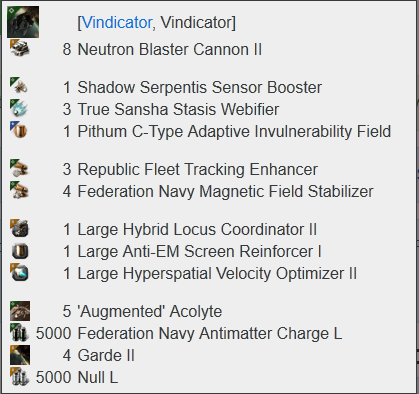
\includegraphics[]{fittingwindow-example.png}
\end{figure}

\subsection{Inviting}
\begin{figure}[h]
	\centering
	\caption{Approved Waitlist Entry}
	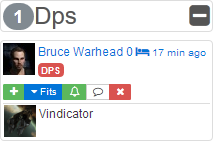
\includegraphics{approved-entry.png}
\end{figure}

\begin{itemize}
	\item The Buttons \picfits behaves exactly the same as in a X-UP Entry\ref{pic:xup-entry}.
	\item \piccross removes them from the 3 type lists (dps/sniper/logi) but NOT from the x-up list.
	\item \picbell Sends the Notification (Gong) and a TeamSpeak poke if their Charactername matches exactly (case sensitive and no additions). The message contains the Waitlistname they were gonged from. This is mostly there in case CCP fucks up the api or you need a person for something else then inviting!
	\item \picinvite sends an invite to the person using eveapi. The character is invited to the specific squad. This triggers the Notification and TS-Poke, in the TS-Poke it is written which waitlist they were invited from (dps/sniper/logi).
\end{itemize}
TS-Pokes can be disabled on the X-UP Form, they are enabled by default.
Inviting some one sets off a timer that check for the invite beeing accepted and then removes a found character from the Waitlist.

\subsection{Fleet Shutdown}
\picfleetsetting
\begin{itemize}
	\item If you are the last fleet of for this list, set Status to "Down" and un-tick the X-UP Open box, then click \picset.
	\item Remove yourself from the FC/Fleet Manager field by pressing \piccross to the right of your name.
	\item Remove your Fleet from the Fleetlist by pressing \picremove.
\end{itemize}

\subsection{Changing Fleet's assigned Waitlist}
\picassignedfleet



Make sure the Fleet-Type you want to change to, has a X-UPs open and press \picchangetype \xspace next to your Fleet.
You will get a Screen like this \picsettype where you can select the Fleet-Type you want to change to, if a Waitlist is not Open, it's type will not be listed here!
Press \picchangetype \xspace and your fleet should now be listed under the other Waitlistsettings.
FCs needs to manually remove them selves from the old Waitlistgroup-Settings and add himself to the ones of the new Type.

\subsection{TeamSpeak Settings}
These Settings are used for the TS-Poke.

Should only be changed if the TS-Server is changing (e.g. going to a backup TS)


\picteamspeaksettings

Select a TS-Server from the Dropdown and press \picchangets \xspace to make the TS-Bot change server 


\subsection{Setting your Waitlist Character}
\begin{figure}[H]
	\caption{Settings -\textgreater \xspace Own Settings}
	\picownsettings
\end{figure}
Under \texttt{Default Character} fill in the character name you want to use, then press \picapply .

\section{Administrator Guide}
\subsection{Ship Classification}
\subsubsection{General Overview}

Ship Classification is used to sort submitted fits into the different waitlists and assign tags to them. There are Collections and Checks. A Collection contains Checks and Each Group of Waitlists can only have one Collection assigned to it while each Collection can also only be allotted to one Waitlist Group.

\subsubsection{Collection}
A Collection, is a Collection of Check that will be applied to fittings.
Each Collection has it's own name and Waitlist-Group it assigned to. Further they have a default Waitlist and Tag, these get assigned to Fittings if none of the Checks match.

\subsubsection{Check}
Each Check is part of a Collection.
They have a Name that is only there to make them more easy to be identified by humans.
Further they have target Waitlist and Tag that is assigned to Fittings which match the Checks rules.

\paragraph{Ordering of Rules}
Each Rule has an order Attribute which defines the order in which they are executed.
Lower Order numbers get applied first.
If more then one rule have the same priority then module rules are applied before hull rules.
If more then one hull rules are of the same priority they are applied in arbitrary order.
If more then one module rule are of the same priority the get applied in the same pass. For more info \nameref{para:module_rules}

\paragraph{Hull Rules}
There is 3 different types of rules that match against the hull type. You can match by type-id, inventory-group-id or market-group-id.

\paragraph{Module Rules}\label{para:module_rules}
There is two different types of rules for matching against highslot modules.
They can be matched against type-id or market-group-id.

Additionally for these rules you can set restrictions by type-id, inventory-group-id or market-group-id regarding the hull these modules are on. If there is no restriction set the rule applies for all hulls.
If there is multiple restrictions set the hull must match ANY of them to be applied.

For module rules there is an modifier attribute that allows to have a specific rule be worth more then an other.
When module rules are applied, all the module rules with the same priority get applied at random order, while a module gets filtered out after being matched by one rule. When a type-id is matched it gets the modifier of the rule assigned as value.


After all highslot modules are check the module that accumulated the highest value is selected.
This way there could be rules for e.g. Blaster with a modifier of 1.00 and a rule for Large Remove Shield Booster with a modifier of 2.00. Now if a Vindicator has 4 Blaster and 3 Remote Shield Booster the result would be a score of 4.00 for the Blaster rule and a 6 for the Remote Shield Booster.
And in the end it would get assigned the Tag and Waitlist of the Remote Shield Booster rule.

If the value is not at least 4.00 the result is treated as if the rules would not have matched.

\end{document}
